% !TEX program = xelatex
\documentclass[11pt,a4paper]{article}
\usepackage[a4paper,left=29mm,right=29mm,top=24mm,bottom=25mm,headheight=22pt]{geometry}
\usepackage{fontspec}
\usepackage{xeCJK}
\usepackage{amsmath}
\usepackage{unicode-math}
\usepackage{xcolor}
\usepackage{graphicx}
\usepackage{booktabs,longtable,array,calc}
\usepackage{caption}
\usepackage{titlesec}
\usepackage{fancyhdr}
\usepackage{needspace}
\usepackage{enumitem}
\usepackage[unicode,pdfusetitle,hidelinks]{hyperref}
\usepackage{bookmark}

\setmainfont{STIXTwoText}[
  Extension=.otf,UprightFont=*-Regular,BoldFont=*-Bold,
  ItalicFont=*-Italic,BoldItalicFont=*-BoldItalic]
\setmathfont{STIXTwoMath-Regular.otf}
\setCJKmainfont{SimSun}[BoldFont=SimHei,ItalicFont=KaiTi]
\setCJKsansfont{SimHei}
\xeCJKsetup{PunctStyle=banjiao,CJKecglue={\hskip 0.16em plus 0.06em minus 0.04em}}

\definecolor{ink}{HTML}{202B32}
\definecolor{accent}{HTML}{275866}
\definecolor{quiet}{HTML}{52646B}
\definecolor{rulegray}{HTML}{BAC8CA}
\definecolor{figureblue}{HTML}{2563EB}
\definecolor{tailgold}{HTML}{A95A04}
\AtBeginDocument{%
  \color{ink}%
  \fontsize{11.25}{17.1}\selectfont
  \setlength{\abovedisplayskip}{7pt plus 2pt minus 2pt}%
  \setlength{\belowdisplayskip}{7pt plus 2pt minus 2pt}%
  \setlength{\abovedisplayshortskip}{5pt plus 2pt minus 1pt}%
  \setlength{\belowdisplayshortskip}{6pt plus 2pt minus 1pt}}
\setlength{\parindent}{0pt}
\setlength{\parskip}{5pt plus 1pt minus 0.6pt}
\setlength{\emergencystretch}{2em}
\widowpenalty=10000
\clubpenalty=10000
\displaywidowpenalty=10000
\interdisplaylinepenalty=10000
\raggedbottom

\setcounter{secnumdepth}{0}
\setcounter{tocdepth}{2}
\titleformat{\section}{\Large\bfseries\color{accent}}{}{0pt}{}
\titleformat{\subsection}{\large\bfseries\color{ink}}{}{0pt}{}
\titleformat{\subsubsection}{\normalsize\bfseries\color{ink}}{}{0pt}{}
\titlespacing*{\section}{0pt}{21pt plus 3pt}{5pt}
\titlespacing*{\subsection}{0pt}{13pt plus 3pt}{3pt}
\titlespacing*{\subsubsection}{0pt}{10pt plus 2pt}{2pt}
\setlist[itemize]{leftmargin=1.45em,itemsep=1pt,topsep=3pt,parsep=0pt}
\providecommand{\tightlist}{\setlength{\itemsep}{0pt}\setlength{\parskip}{0pt}}

\renewcommand{\figurename}{图}
\renewcommand{\tablename}{表}
\captionsetup{font=small,labelfont={bf,color=accent},labelsep=quad,hypcap=false,
  justification=raggedright,singlelinecheck=false,skip=6pt}
\captionsetup[table]{position=top}
\renewcommand{\arraystretch}{1.18}
\setlength{\LTpre}{7pt}
\setlength{\LTpost}{7pt}
\setlength{\LTcapwidth}{\textwidth}
\newenvironment{readerfigure}
  {\par\addvspace{7pt}\noindent\begin{minipage}{\linewidth}\centering\small}
  {\end{minipage}\par\addvspace{9pt}}
\newcommand{\figuretitle}[1]{\par{\bfseries\color{accent}#1}\par\smallskip}
\newcommand{\legendmark}[1]{\textcolor{#1}{\rule[.22ex]{1.1em}{1.1pt}}}
\newenvironment{readerquestion}[1]
  {\par\addvspace{9pt}\noindent\begin{minipage}{\linewidth}%
   {\color{rulegray}\hrule}\vspace{5pt}%
   {\small\bfseries\color{accent}#1}\par\smallskip\small}
  {\end{minipage}\par}

\pagestyle{fancy}
\fancyhf{}
\fancyhead[L]{\small\color{quiet}科研准备学习路线}
\fancyhead[R]{\small\color{quiet}IV-A \enspace Financial Time Series}
\fancyfoot[R]{\small\color{quiet}\thepage}
\renewcommand{\headrulewidth}{0.3pt}
\makeatletter
\renewcommand{\headrule}{\hbox to\headwidth{\color{rulegray}\leaders\hrule height \headrulewidth\hfill}}
\makeatother

\renewcommand{\contentsname}{选读目录}
\title{科研准备学习路线 · 数学读本样张}
\author{}
\date{}
\hypersetup{pdfsubject={IV-A Financial Time Series \& Data Generating Process},
            pdflang={zh-CN}, bookmarksnumbered=false}

\begin{document}
\thispagestyle{empty}
\pdfbookmark[0]{样张导读}{prototype}
\vspace*{9mm}

{\color{accent}\bfseries X Program \#161\enspace·\enspace Research Preparation\par}
\vspace{4pt}
{\fontsize{30}{39}\selectfont\bfseries 科研准备学习路线\par}
{\large 数学读本样张\par}
\vspace{10pt}
{\color{rulegray}\hrule}
\vspace{9pt}

{\large\bfseries IV-A \enspace Financial Time Series \& Data Generating Process\par}
\vspace{2pt}
本样张取自原对话中从 §6.2 到 §7.3 的连续补讲。保留原文的中英术语、公式、推导和例表。图中的交互控件以标明参数的静态画面呈现。

% Original passages from source messages 05 (78–87) and 57 (complete).
\begin{readerquestion}{研究准备中的提问}
讨论：

\begin{itemize}
\tightlist
\item
  Financial Time Series 的统计特点
\item
  Non-stationarity 与 Regime Shifts
\item
  Backtesting Overfitting
\item
  Transaction Costs 和现实交易约束
\item
  Sharpe Ratio 等常见评估指标
\item
  为什么金融模型的样本外评估更困难？
\end{itemize}

不需要一开始就深入复杂的衍生品定价理论。
\end{readerquestion}

\begin{readerquestion}{续读请求}
欸上一条输出完了吗？看起来好像在6.2停住了？你从6.2开始再把后面的补齐
\end{readerquestion}


\vspace{7pt}
\tableofcontents

\clearpage
% Generated by scripts/build_excerpt.py
\hypertarget{stylized-facts-of-financial-returns}{%
\section{6. Stylized Facts of Financial Returns}\label{stylized-facts-of-financial-returns}}

\hypertarget{volatility-clusteringux6ce2ux52a8ux7387ux805aux96c6}{%
\subsection{6.2 Volatility Clustering（波动率聚集）}\label{volatility-clusteringux6ce2ux52a8ux7387ux805aux96c6}}

金融市场中的高波动通常倾向于连续出现，低波动时期也可能持续一段时间。

\begin{readerfigure}
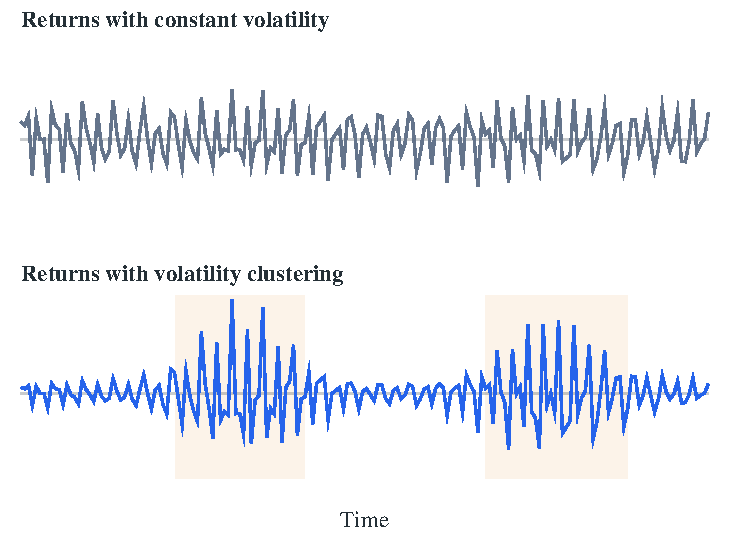
\includegraphics[width=0.72\linewidth]{figures/volatility.pdf}
\captionof{figure}{合成示意：下方序列的收益率方向难以预测，但波动幅度具有明显的持续性。}
\end{readerfigure}

因此，在金融数据中，我们可能同时观察到：
\[\operatorname{Corr}(r_t,r_{t+h})\approx0,\]

但：
\[\operatorname{Corr}(|r_t|,|r_{t+h}|)>0,\]

或者：
\[\operatorname{Corr}(r_t^2,r_{t+h}^2)>0.\]

这意味着：

\textbf{收益率本身可能不具有明显的线性可预测性，但其波动程度具有可预测性。}

\begin{readerfigure}
\figuretitle{Typical Financial Return ACF}
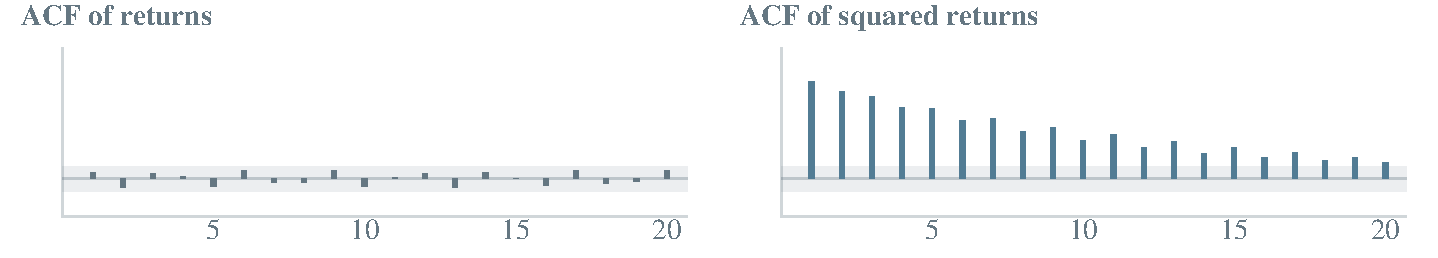
\includegraphics[width=0.72\linewidth]{figures/acf.pdf}
\captionof{figure}{典型形态的教学示意，非实际市场数据。原始收益率的自相关接近零，平方收益率的自相关则可能缓慢衰减。}
\end{readerfigure}

\hypertarget{ux4e00ux4e2aux4e25ux683cux7684ux6982ux7387ux53cdux4f8b}{%
\subsection{6.3 一个严格的概率反例}\label{ux4e00ux4e2aux4e25ux683cux7684ux6982ux7387ux53cdux4f8b}}

为了进一步理解为什么 Uncorrelated 不等于 Independent，我们构造一个非常简单的随机过程。

设：
\[Z_t\overset{\mathrm{i.i.d.}}{\sim}\mathcal N(0,1),\]

并定义：
\[r_t=Z_tZ_{t-1}.\]

首先，由独立性：
\[\mathbb E[r_t]
=
\mathbb E[Z_t]\mathbb E[Z_{t-1}]
=0.\]

\hypertarget{proposition-1-returns-are-uncorrelated}{%
\subsubsection{Proposition 1 --- Returns are uncorrelated}\label{proposition-1-returns-are-uncorrelated}}

相邻收益率的协方差为：
\[\begin{aligned}
\operatorname{Cov}(r_t,r_{t+1})
&=\mathbb E[r_tr_{t+1}]\\
&=\mathbb E[Z_t^2Z_{t-1}Z_{t+1}]\\
&=\mathbb E[Z_t^2]
\mathbb E[Z_{t-1}]
\mathbb E[Z_{t+1}]\\
&=0.
\end{aligned}\]

因此：
\[\boxed{
\operatorname{Cov}(r_t,r_{t+1})=0.
}\]

\hypertarget{proposition-2-squared-returns-are-correlated}{%
\subsubsection{Proposition 2 --- Squared returns are correlated}\label{proposition-2-squared-returns-are-correlated}}

现在考察平方收益率：
\[r_t^2=Z_t^2Z_{t-1}^2.\]

由于标准正态分布满足：
\[\mathbb E[Z_t^2]=1,
\qquad
\mathbb E[Z_t^4]=3,\]

所以：
\[\mathbb E[r_t^2]=1.\]

进一步：
\[\begin{aligned}
&\operatorname{Cov}(r_t^2,r_{t+1}^2)\\
&=\mathbb E[r_t^2r_{t+1}^2]
-\mathbb E[r_t^2]\mathbb E[r_{t+1}^2]\\
&=\mathbb E[Z_t^4Z_{t-1}^2Z_{t+1}^2]-1\\
&=\mathbb E[Z_t^4]
\mathbb E[Z_{t-1}^2]
\mathbb E[Z_{t+1}^2]-1\\
&=3-1\\
&=2.
\end{aligned}\]

于是：
\[\boxed{
\operatorname{Cov}(r_t^2,r_{t+1}^2)=2>0.
}\]

我们甚至可以进一步计算其平方收益率的相关系数。

由于：
\[\begin{aligned}
\operatorname{Var}(r_t^2)
&=\mathbb E[r_t^4]-\mathbb E[r_t^2]^2\\
&=3\times3-1\\
&=8,
\end{aligned}\]

因此：
\[\operatorname{Corr}(r_t^2,r_{t+1}^2)
=
\frac28
=
\frac14.\]

最终得到：
\[\boxed{
\begin{aligned}
\operatorname{Corr}(r_t,r_{t+1})&=0,\\
\operatorname{Corr}(r_t^2,r_{t+1}^2)&=0.25.
\end{aligned}
}\]

这严格证明了一个随机过程可以不存在收益率的线性相关性，却存在波动幅度的统计依赖。

当然，这只是一个概率论反例，而不是完整的金融市场模型。

\hypertarget{arch-and-garch}{%
\subsection{6.4 ARCH and GARCH}\label{arch-and-garch}}

为了描述 Volatility Clustering，金融计量经济学发展出了两种经典模型：

\begin{longtable}[]{@{}
  >{\raggedright\arraybackslash}p{(\columnwidth - 4\tabcolsep) * \real{0.16}}
  >{\raggedright\arraybackslash}p{(\columnwidth - 4\tabcolsep) * \real{0.67}}
  >{\raggedleft\arraybackslash}p{(\columnwidth - 4\tabcolsep) * \real{0.17}}@{}}
\caption{ARCH 与 GARCH}\tabularnewline
\toprule
Model & Full Name & Year \\
\midrule
\endfirsthead
\toprule
Model & Full Name & Year \\
\midrule
\endhead
ARCH & Autoregressive Conditional Heteroskedasticity & 1982 \\
GARCH & Generalized ARCH & 1986 \\
\bottomrule
\end{longtable}

目前只需要掌握 GARCH(1,1) 的基本结构。

\hypertarget{model-definition}{%
\subsubsection{Model Definition}\label{model-definition}}

首先定义收益率：
\[r_t=\mu+\varepsilon_t,\]

其中：
\[\varepsilon_t=\sigma_tZ_t,\]

且 \(Z_t\) 是均值为 0、方差为 1 的 IID Innovation，并独立于过去的信息。

条件方差由下式决定：
\[\boxed{
\sigma_t^2
=
\omega
+a\varepsilon_{t-1}^2
+b\sigma_{t-1}^2
}\]

其中：
\[\omega>0,\qquad a,b\geq0.\]

\begin{longtable}[]{@{}
  >{\raggedright\arraybackslash}p{(\columnwidth - 2\tabcolsep) * \real{0.23}}
  >{\raggedright\arraybackslash}p{(\columnwidth - 2\tabcolsep) * \real{0.77}}@{}}
\caption{GARCH 模型的参数}\tabularnewline
\toprule
Parameter & Interpretation \\
\midrule
\endfirsthead
\toprule
Parameter & Interpretation \\
\midrule
\endhead
\(\omega\) & 方差方程的常数项 \\
\(a\) & 对近期市场冲击的敏感程度 \\
\(b\) & 历史条件方差的持续程度 \\
\(a+b\) & 波动冲击在条件方差预测中的持续性 \\
\bottomrule
\end{longtable}

\begin{readerfigure}
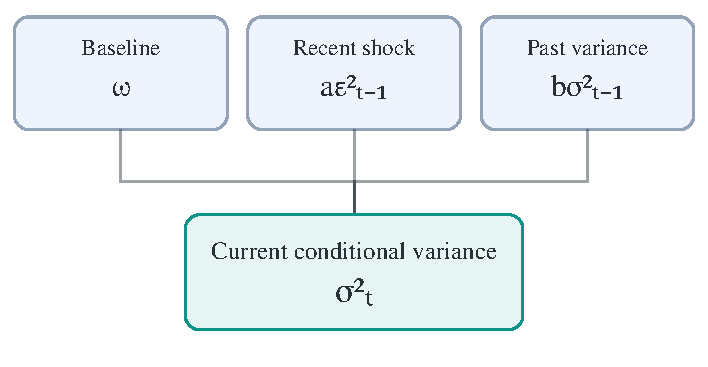
\includegraphics[width=0.8\linewidth]{figures/garch-mechanism.pdf}
\captionof{figure}{GARCH(1,1) 条件方差的组成}
\end{readerfigure}

GARCH 的基本思想是：当前波动率不仅取决于最近一次市场冲击，还受到此前波动率的影响。

\hypertarget{proposition-unconditional-variance}{%
\subsubsection{Proposition --- Unconditional Variance}\label{proposition-unconditional-variance}}

假设存在具有有限二阶矩的平稳解，并满足：
\[a+b<1.\]

对条件方差方程两侧取期望：
\[\mathbb E[\sigma_t^2]
=
\omega
+a\mathbb E[\varepsilon_{t-1}^2]
+b\mathbb E[\sigma_{t-1}^2].\]

根据 Law of Total Expectation：
\[\begin{aligned}
\mathbb E[\varepsilon_{t-1}^2]
&=\mathbb E[
\mathbb E[\varepsilon_{t-1}^2
\mid\mathcal F_{t-2}]
]\\
&=\mathbb E[\sigma_{t-1}^2].
\end{aligned}\]

因此：
\[\mathbb E[\sigma_t^2]
=
\omega+(a+b)\mathbb E[\sigma_{t-1}^2].\]

由平稳性：
\[\mathbb E[\sigma_t^2]
=
\mathbb E[\sigma_{t-1}^2].\]

于是：
\[\boxed{
\mathbb E[\sigma_t^2]
=
\frac{\omega}{1-a-b}.
}\]

这同时也是上述模型中收益率的无条件方差。

\hypertarget{volatility-persistence}{%
\subsubsection{Volatility Persistence}\label{volatility-persistence}}

设长期方差为：
\[\bar\sigma^2=\frac{\omega}{1-a-b}.\]

条件方差预测向长期方差回归的速度主要由 \(a+b\) 决定。

\begin{readerfigure}
\figuretitle{GARCH --- Volatility Shock Persistence}
\begin{minipage}[t]{.318\linewidth}\centering \textbf{\(a+b=0.50\)}\par\smallskip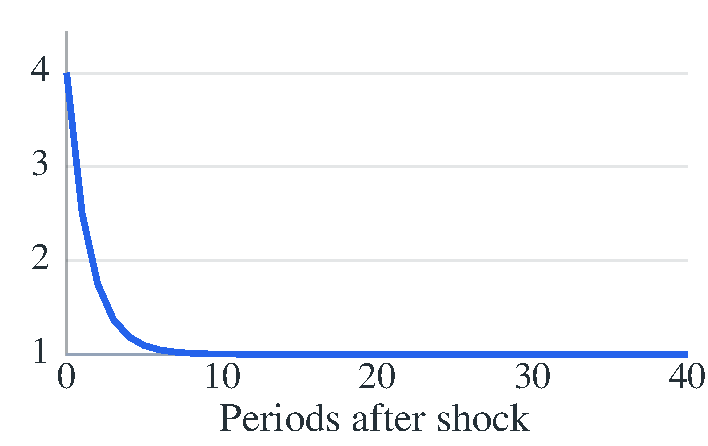
\includegraphics[width=\linewidth]{figures/garch-persistence-0.50.pdf}\end{minipage}\hfill\begin{minipage}[t]{.318\linewidth}\centering \textbf{\(a+b=0.90\)}（默认）\par\smallskip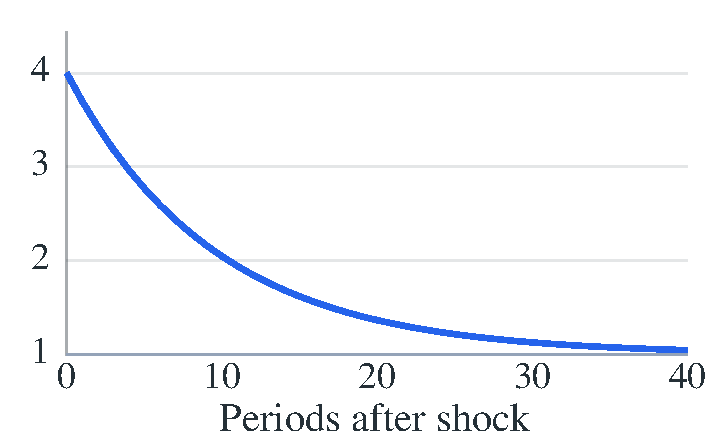
\includegraphics[width=\linewidth]{figures/garch-persistence-0.90.pdf}\end{minipage}\hfill\begin{minipage}[t]{.318\linewidth}\centering \textbf{\(a+b=0.99\)}\par\smallskip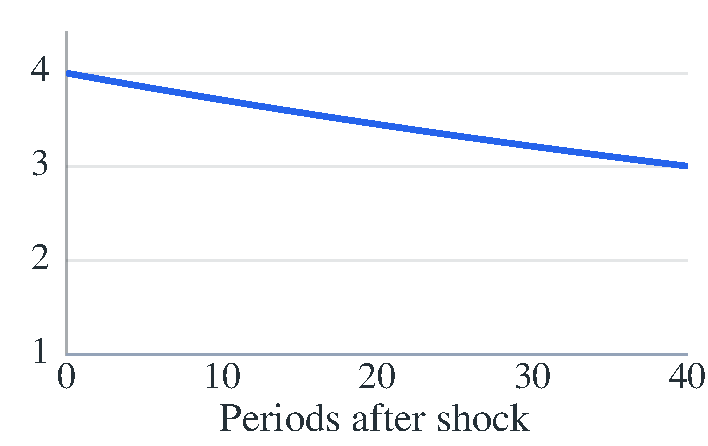
\includegraphics[width=\linewidth]{figures/garch-persistence-0.99.pdf}\end{minipage}

\smallskip
\begin{tabular}{@{}lrrr@{}}
\toprule
\(a+b\) & 0.50 & 0.90 & 0.99 \\
\midrule
Shock half-life（连续插值，Periods） & 1.00 & 6.58 & 68.97 \\
Remaining shock after 20 periods & 0.0\% & 12.2\% & 81.8\% \\
\bottomrule\end{tabular}
\captionof{figure}{归一化教学模型：长期方差为 1，初始超额方差为 3。曲线描述条件方差预测的恢复过程。}
\end{readerfigure}

这里有一个相当 Nontrivial 的观点：

\textbf{Conditional Variance 随时间变化，并不意味着 Unconditional Variance 随时间变化。}

GARCH 可以同时具有：

\begin{itemize}
\tightlist
\item
  Time-varying Conditional Variance；
\item
  Constant Unconditional Variance；
\item
  Weak Stationarity。
\end{itemize}

所以：
\[\boxed{
\text{Volatility Clustering}
\not\Rightarrow
\text{Non-stationarity}.
}\]

这一点非常容易混淆。

\hypertarget{heavy-tailsux539aux5c3eux5206ux5e03}{%
\section{7. Heavy Tails（厚尾分布）}\label{heavy-tailsux539aux5c3eux5206ux5e03}}

\hypertarget{gaussian-assumption-ux7684ux5c40ux9650}{%
\subsection{7.1 Gaussian Assumption 的局限}\label{gaussian-assumption-ux7684ux5c40ux9650}}

我们此前大量使用 Normal Distribution，因为它具有非常好的数学性质。

但是，现实金融收益率经常表现出比正态分布更厚的尾部，即极端观测值出现的概率比 Gaussian Model 所预期的更高。

\begin{readerfigure}
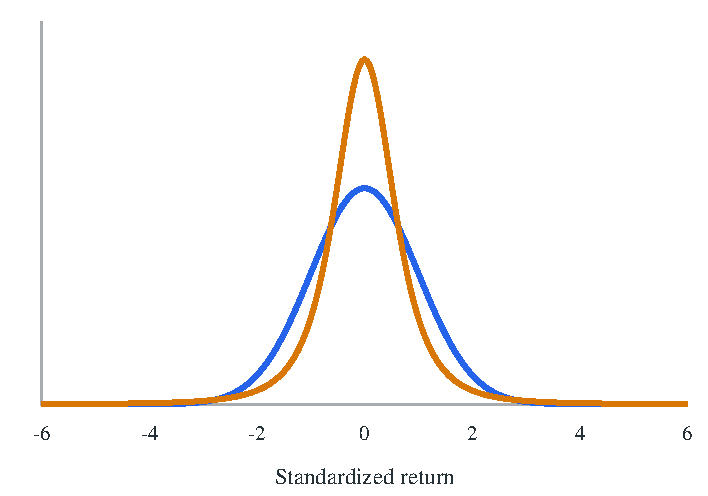
\includegraphics[width=0.7\linewidth]{figures/densities.pdf}
\par\smallskip \legendmark{figureblue}\enspace Standard Normal\qquad \legendmark{tailgold}\enspace Standardized Student's t (ν=3)
\captionof{figure}{两种分布均具有零均值和单位方差，但尾部概率存在显著差异。}
\end{readerfigure}

例如，我们比较 Standard Normal Distribution 与标准化为单位方差的 Student's t Distribution（自由度为 3）。

\begin{longtable}[]{@{}
  >{\raggedright\arraybackslash}p{(\columnwidth - 4\tabcolsep) * \real{0.43}}
  >{\raggedleft\arraybackslash}p{(\columnwidth - 4\tabcolsep) * \real{0.25}}
  >{\raggedleft\arraybackslash}p{(\columnwidth - 4\tabcolsep) * \real{0.32}}@{}}
\caption{双侧理论尾部概率}\tabularnewline
\toprule
Extreme Event & Normal & Standardized \(t_3\) \\
\midrule
\endfirsthead
\toprule
Extreme Event & Normal & Standardized \(t_3\) \\
\midrule
\endhead
超过 3 个标准差 & 0.270\% & 1.385\% \\
超过 5 个标准差 & 0.0000573\% & 0.324\% \\
\bottomrule
\end{longtable}

以上均为双侧理论尾部概率。

\begin{readerfigure}
\figuretitle{Probability of a 5-standard-deviation event}
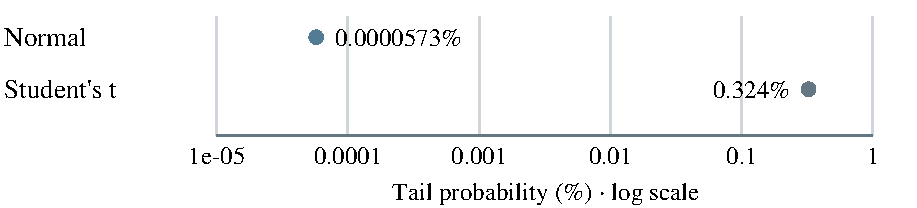
\includegraphics[width=0.73\linewidth]{figures/tail-probability.pdf}
\par\medskip\textcolor{tailgold}{\textbf{约 5,650 倍}}
\captionof{figure}{即使均值和方差完全相同，极端事件概率也可能存在数量级差异。}
\end{readerfigure}

这也是为什么仅仅比较 Mean 和 Variance，可能不足以充分描述金融数据的风险特征。

\Needspace{10\baselineskip}
\hypertarget{moment-existenceux77e9ux7684ux5b58ux5728ux6027}{%
\subsection{7.2 Moment Existence（矩的存在性）}\label{moment-existenceux77e9ux7684ux5b58ux5728ux6027}}

Student's t Distribution 具有一个值得关注的数学性质。

对于：
\[X\sim t_\nu,\]

其 \(p\) 阶绝对矩存在的条件为：
\[\boxed{
\mathbb E[|X|^p]<\infty
\iff p<\nu,
\qquad p>0.
}\]

\begin{longtable}[]{@{}
  >{\raggedright\arraybackslash}p{(\columnwidth - 6\tabcolsep) * \real{0.32}}
  >{\raggedright\arraybackslash}p{(\columnwidth - 6\tabcolsep) * \real{0.19}}
  >{\raggedright\arraybackslash}p{(\columnwidth - 6\tabcolsep) * \real{0.22}}
  >{\raggedright\arraybackslash}p{(\columnwidth - 6\tabcolsep) * \real{0.27}}@{}}
\caption{Student's t Distribution 的矩}\tabularnewline
\toprule
Degrees of Freedom & Mean & Variance & Fourth Moment \\
\midrule
\endfirsthead
\toprule
Degrees of Freedom & Mean & Variance & Fourth Moment \\
\midrule
\endhead
\(\nu=1\) & 不存在 & 不存在 & 不存在 \\
\(\nu=2\) & 存在 & 不存在 & 不存在 \\
\(\nu=3\) & 存在 & 存在 & 不存在 \\
\(\nu=5\) & 存在 & 存在 & 存在 \\
\bottomrule
\end{longtable}

其中：
\[t_1=\text{Cauchy Distribution}.\]

也就是此前 Probability 中学习过的 Cauchy Distribution。

\hypertarget{proof-sketch}{%
\subsubsection{Proof Sketch}\label{proof-sketch}}

Student's t Distribution 的概率密度为：
\[f_\nu(x)
=
\frac{
\Gamma((\nu+1)/2)
}{
\sqrt{\nu\pi}\Gamma(\nu/2)
}
\left(1+\frac{x^2}{\nu}\right)^{-(\nu+1)/2}.\]

当 \(|x|\to\infty\) 时：
\[f_\nu(x)\asymp |x|^{-(\nu+1)}.\]

因此，绝对矩积分的尾部行为为：
\[\int^\infty x^pf_\nu(x)\,\mathrm dx
\asymp
\int^\infty x^{p-\nu-1}\,\mathrm dx.\]

根据 Improper Integral 的收敛条件：
\[p-\nu-1<-1,\]

即：
\[\boxed{p<\nu.}\]

\Needspace{13\baselineskip}
\hypertarget{heavy-tails-ux5bf9ux7edfux8ba1ux5b66ux4e60ux7684ux5f71ux54cd}{%
\subsection{7.3 Heavy Tails 对统计学习的影响}\label{heavy-tails-ux5bf9ux7edfux8ba1ux5b66ux4e60ux7684ux5f71ux54cd}}

现在回顾 Part II 中使用过的几个数学工具。

\begin{longtable}[]{@{}
  >{\raggedright\arraybackslash}p{(\columnwidth - 4\tabcolsep) * \real{0.32}}
  >{\raggedright\arraybackslash}p{(\columnwidth - 4\tabcolsep) * \real{0.32}}
  >{\raggedright\arraybackslash}p{(\columnwidth - 4\tabcolsep) * \real{0.36}}@{}}
\caption{厚尾对统计工具的影响}\tabularnewline
\toprule
Statistical Tool & Relevant Assumption & Potential Problem \\
\midrule
\endfirsthead
\toprule
Statistical Tool & Relevant Assumption & Potential Problem \\
\midrule
\endhead
Chebyshev Inequality & Finite Variance & 方差可能不存在 \\
Classical IID CLT & Finite Variance & 极限分布可能不是正态 \\
Hoeffding Inequality & Bounded Variables & 收益率或损失函数可能无界 \\
Sample Variance Inference & 通常涉及高阶矩条件 & 方差估计本身可能非常不稳定 \\
Standard Bootstrap & 依赖统计量及分布条件 & 厚尾可能影响重采样推断 \\
\bottomrule
\end{longtable}

尤其需要注意一种情况：

假设预测误差具有有限二阶矩，却没有有限四阶矩。

那么对于 Squared Loss：
\[L=\varepsilon^2,\]

我们可能有：
\[\mathbb E[L]=\mathbb E[\varepsilon^2]<\infty,\]

但：
\[\operatorname{Var}(L)
=
\mathbb E[\varepsilon^4]
-\mathbb E[\varepsilon^2]^2
=\infty.\]

也就是说，\textbf{Population MSE 可以存在，但经验 MSE 的方差可能不存在。}

这使得两个模型之间微小的 MSE Improvement 更难被可靠识别。

对于 Financial RSI，Agent 可能不断根据高度不稳定的 Evaluation Score 修改自身，并将偶然出现的极端结果误认为真实研究规律。

当然，金融数据具有厚尾，并不意味着它一定没有有限方差。上述结论取决于具体 DGP 与所使用的损失函数。


\end{document}
